\documentclass{article}

\usepackage[spanish]{babel}
\usepackage[utf8]{inputenc}
\usepackage[T1]{fontenc}
\usepackage{graphicx}
\usepackage{hyperref}
\usepackage{courier}
\usepackage{listings}
\usepackage{xcolor}
\usepackage{blindtext}
\usepackage{scrextend}
\usepackage[document]{ragged2e}
\usepackage{multicol}
\usepackage{pgfgantt}
\usepackage{mathtools}
\usepackage{minted}
\usepackage{tikz}
\usepackage{longtable}
\usepackage{algorithm}
\usepackage[noend]{algpseudocode}
\usepackage{amsmath}
\usepackage{wrapfig,lipsum,booktabs}
\usepackage{fontspec}
 % % % % % % % %

\setmainfont{Calibri}

\hypersetup{
	colorlinks,
	linkcolor={blue!60!black},
	citecolor={blue!50!black},
	urlcolor={blue!80!black}
}

\usetikzlibrary{positioning,fit,calc}

\usemintedstyle{pastie}

\usepackage{array}
\newcolumntype{L}[1]{>{\raggedright\let\newline\\\arraybackslash\hspace{0pt}}m{#1}}
\newcolumntype{C}[1]{>{\centering\let\newline\\\arraybackslash\hspace{0pt}}m{#1}}
\newcolumntype{R}[1]{>{\raggedleft\let\newline\\\arraybackslash\hspace{0pt}}m{#1}}

\def\labelitemi{\textbf{--}}

\usepackage{anysize}
\marginsize{2.54cm}{2.54cm}{2.54cm}{2.54cm}

\usepackage{setspace}
%\onehalfspacing
\doublespacing

\makeatletter
\newcommand*{\MoveFitHeight}[1]{%
	\pgfmathsetlengthmacro\fit@inner@sep{%
		\pgfkeysvalueof{/pgf/inner xsep}%
	}%
	\pgfmathsetlengthmacro\fit@text@height{%
		\tikz@text@height
	}%
	\kern-\fit@inner@sep\relax
	\raisebox{\fit@text@height}[0pt][0pt]{#1}%
}
\makeatother

\newcommand{\bigO}[1]{$O({#1})$}

\setlength{\columnsep}{1cm}

%En caso de que LaTeX separe las palabras con - de manera incorrecta, usar
%\hyphenation{deci-sión,e-xa-men, otras palabras....}

\begin{document}
%--% Portada %------------------------------------------%
\centerline{Universidad de Carabobo}
\centerline{Facultad de Ciencia y Tecnologia}
\centerline{Sistemas Operativos}
\vspace{7cm}
\begin{centering}
	\hrule 	\vspace{0.4cm}
	{ \Huge \bfseries Algoritmos de Remoción de Páginas \\[0.4cm] }
	\hrule \vfill
\end{centering}
\vfill
\centerline{Victor Tortolero, 24.569.609}
\centerline{\today}
\newpage
%-------------------------------------------------------%
	
{\centering \section*{Algoritmos de Remoción de Páginas}}
Cuando ocurre un fallo de página, el sistema operativo tiene que elegir una página para desalojarla (eliminarla de memoria) y hacer espacio
para la página entrante. Si la página a eliminar se modificó mientras estaba en memoria, deve voler a escribirse en disco para
actualizar la copia del mismo. No obstante, si la pagina no se ha modificado, la copia ya está actualizada y no se necesita rescribir.

Aunque seria posible elegir una pagina al azar para desalojarla en cada fallo de página, el rendimiento del sistema es mucho mayor si se selecciona una página que no sea de uso frecuente. Si se elimina una pagina de uso frecuente, tal vez tenga que traerse de vuelta rapidamente, lo cual produce una sobrecarga adicional.

{\centering \section*{Algoritmo de reemplazo de páginas óptimo}}
En este algoritmo, cada pagina se etiqueta con el numero de instrucciones que se ejecutaran antes de que se referencie
por primera vez esa pagina. La pagina con la etiqueta mas alta es la que debe eliminarse al ocurrir un fallo de pagina.
Si una página no se va a utilizar durante 8 millones de instrucciones y otra no se va a utilizar durante 6 millones de instrucciones, 
al eliminar la primera se enviará el fallo de página que la obtendrá de vuelta lo más lejos posible en el futuro.

Este algoritmo no puede implantarse, ya que al momento del fallo de pagina, el sistema operativo no tiene forma de saber cuándo será la próxima referencia a cada una de las paginas. Se usa solamente para fines de comparación con otros algoritmos.

\begin{figure}[H]
	\centering
	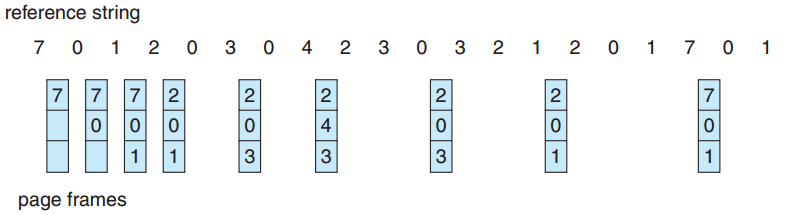
\includegraphics[scale=0.7]{img/optimo.png}
	\caption{Algoritmo Optimo}
\end{figure}

%-------------------------------------------------------------%
{\centering \section*{Algoritmo LRU (Menos recientemente usada)}}
Este algoritmo se basa en descartar la página que no se haya utilizada durante la mayor longitud de tiempo. 
Este algoritmo es usado, y se considera bueno, el problema es implementarlo, ya que podría requerir hardware especializado.

Se puede asociar a cada pagina un campo que cuenta el tiempo en uso, y necesitaríamos un reloj lógico o un contador. Se actualiza este campo cada vez que se hace referencia a la pagina, y se pasa el contenido del reloj a el campo en la pagina correspondiente. El reloj aumenta su cuenta cada vez que ocurre una referencia de memoria. Y se descartaría la pagina con el menor valor el campo de tiempo de uso.

\begin{figure}[H]
	\centering
	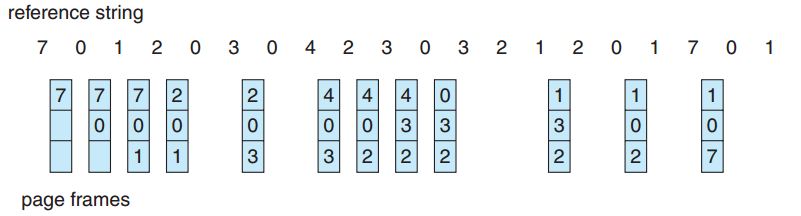
\includegraphics[scale=0.7]{img/lru1.png}
	\caption{Algoritmo LRU con implementado con un contador}
\end{figure}

Otra manera seria tener una pila con los números de las paginas. Cada vez que una pagina se referencia, se saca de la pila y se pone en el tope. De este manera, la pagina mas recientemente usada esta en el tope, y la menos recientemente usada en el fondo de la pila.

\begin{figure}[H]
	\centering
	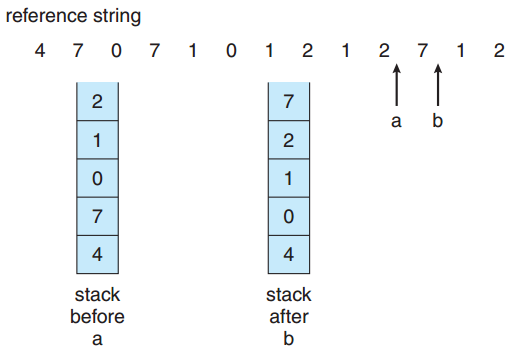
\includegraphics[scale=0.7]{img/lru2.png}
	\caption{Algoritmo LRU implementado con una pila}
\end{figure}


%-------------------------------------------------------------%
{\centering \section*{Algoritmo FIFO (Primero en entrar, Primero en salir)}}
En este algoritmo, el sistema operativo mantiene una lista de todas las páginas actualmente en memoria, en donde la llegada más reciente esta en la parte final y la menos reciente en la parte frontal. Al ocurrir un fallo de pagina, se elimina la pagina que esta en la parte frontal (la que llego hace mas tiempo) y la nueva página se agrega a la parte final de la lista. Este algoritmo no se usa mucho, ya que podría eliminar paginas que se referencien con frecuencia y afectar el rendimiento del sistema.

\begin{figure}[H]
	\centering
	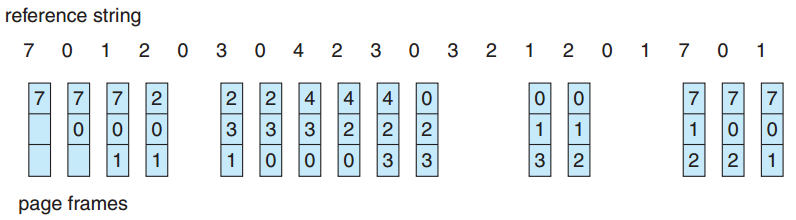
\includegraphics[scale=0.7]{img/fifo.png}
	\caption{Algoritmo FIFO}
\end{figure}


%-------------------------------------------------------------%
{\centering \section*{Algoritmo Segunda Oportunidad}}
Es una modificación del FIFO, en el que al revisar la pagina mas antigua (La que esta el frente de la lista) se revisa su bit $R$ (Indica si se han hecho lecturas o escrituras en la pagina si esta en 1). Si el bit $R$ es 0, la pagina es antigua y no se ha utilizado, por lo que se sustituye de inmediato. Si el bit $R$ es 1, el bit se borra, la pagina se pone al final de la lista de paginas y su tiempo de carga se actualiza, como si acabara de llegar a la memoria, también se restablece su bit $R$, y la búsqueda continua.

\begin{figure}[H]
	\centering
	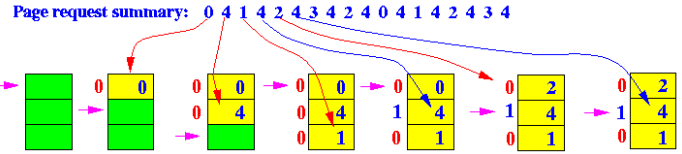
\includegraphics[scale=0.7]{img/sop1.png}
\end{figure}
\begin{figure}[H]
	\centering
	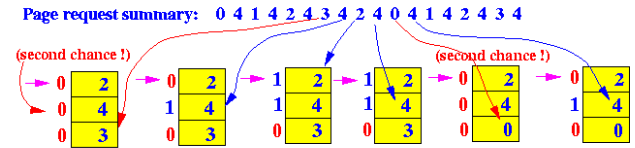
\includegraphics[scale=0.6]{img/sop2.png}
\end{figure}
\begin{figure}[H]
	\centering
	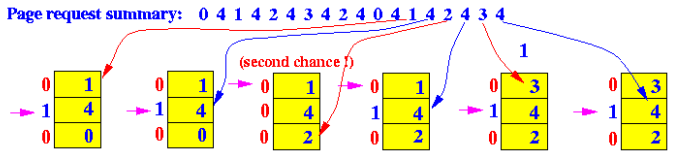
\includegraphics[scale=0.6]{img/sop3.png}
	\caption{Algoritmo Segunda Oportunidad}
\end{figure}


%-------------------------------------------------------------%
{\centering \section*{Algoritmo Reloj}}
Es paracido al segunda oportunidad, pero las paginas se mantienen en una lista circular.
Cuando ocurre un fallo de página, la página a la que apunta la manecilla se inspecciona. Si el bit $R$ es 0, la página se desaloja, se inserta la nueva página en el reloj en su lugar y la manecilla se avanza una posicion. Si $R$ es 1, se pone en 0 y la manecilla se avanza a la siguiente pagina, este proceso se repite hasta encontrar una página con R = 0.

\begin{figure}[H]
	\centering
	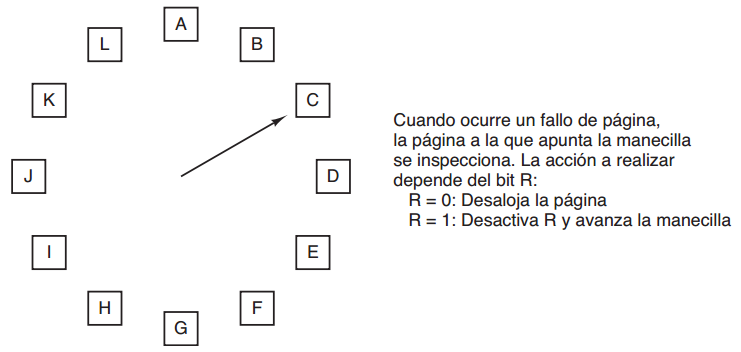
\includegraphics[scale=0.7]{img/reloj.png}
	\caption{Algoritmo Reloj}
\end{figure}

\begin{figure}[H]
	\centering
	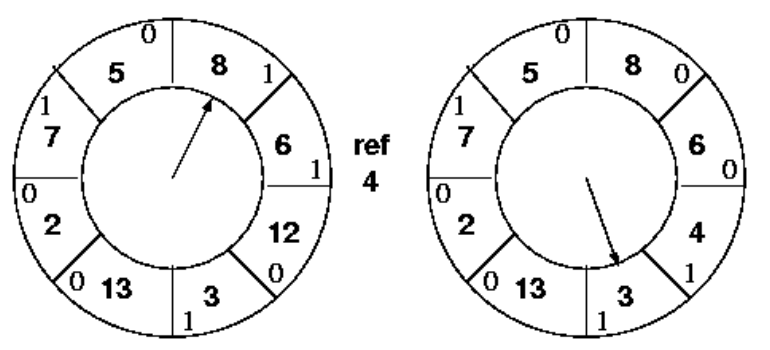
\includegraphics[scale=0.7]{img/reloj2.png}
	\caption{Algoritmo Reloj}
\end{figure}


%-------------------------------------------------------------%
{\centering \section*{Algoritmo NRU (No usadas recientemente)}}
Se usan los 2 bits asociados a cada página, $R$ y $M$. $R$ se prende cava vez que se hace referencia a la página (Lectura o escritura), y M se prende cuando se escribe en la pagina (se modifica). Una vez prendido (o puesto en 1) permanecen así hasta que el sistema operativo lo restablece.

Cuando se inicia un proceso ambos bits ($R$ y $M$) se establecen en 0 mediante el sistema operativo. El bit $R$ se borra en forma periódica (en cada interrupción de reloj) para diferenciar las paginas a las que no se ha hecho referencia recientemente de las que si se han referenciado.

Cuando ocurre un fallo de pagina el sistema operativo inspecciona todas las paginas y las divide en 4 categorías en base en los valores actuales de sus bits $R$ y $M$.

\begin{itemize}
	\item \textbf{Clase 0}: no referenciada, no modificada (R=0, M=0).
	
	\item \textbf{Clase 1}: no referenciada, modificada (R=0, M=1).
	
	\item \textbf{Clase 2}: referenciada, no modificada (R=1, M=0).
	
	\item \textbf{Clase 3}: referenciada, modificada (R=1, M=1).
\end{itemize}

Al ocurrir el fallo de pagina, el algoritmo elimina una página al azar de la clase de menor numeración que no esté vacía. Proporciona un rendimiento que es optimo, pero adecuado.


%-------------------------------------------------------------%
{\centering \section*{Algoritmo Working Set}}
El conjunto de paginas que utiliza un proceso en un momento dado se conoce como su conjunto de trabajo (Working Set). So todo el conjunto de trabajo está en memoria, el proceso se ejecutará sin producir muchos fallos hasta que avance a otra fase de ejecución. La cantidad de tiempo de la CPU que ha utilizado en realidad en un proceso desde que empezó se conoce como tiempo virtual actual. Con esta aproximación, el conjunto de trabajo de un proceso es el conjunto de paginas a las que se han hecho referencia durante los últimos $\tau$ segundos de tiempo virtual.

La idea de este algoritmo es buscar una pagina que no esté en el conjunto de trabajo y desalojarla. Este algoritmo usa el tiempo que se utilizo la página por ultima vez y el bit $R$ (referenciada).

A medida que se procesa cada entrada, se examina el bit R. Si es 1, el tiempo virtual actual se escribe en el campo tiempo de último uso en la tabla de páginas, indicando que la página estaba en uso al momento en que ocurrió el fallo de página. Como se hizo referencia a la página durante el pulso de reloj actual, es evidente que está en el conjunto de trabajo y no es candidata para la eliminación (se supone que $\tau$ abarca varios pulsos de reloj).

Si R es 0, no se ha hecho referencia a la página durante el pulso de reloj actual y puede ser candidata para la eliminación. Para ver si debe o no eliminarse, se calcula su edad (el tiempo virtual
actual menos su tiempo de último uso) y se compara con $\tau$. Si la edad es mayor que $\tau$, la página ya no se encuentra en el conjunto de trabajo y la nueva página la sustituye. La exploración continúa actualizando las entradas restantes.

No obstante, si $R$ es 0 pero la edad es menor o igual que τ, la página está todavía en el conjunto de trabajo. La página se reserva temporalmente, pero se apunta la página con la mayor edad (el menor valor de Tiempo de último uso). Si toda la tabla completa se explora sin encontrar un candidato para desalojar, eso significa que todas las páginas están en el conjunto de trabajo. En ese caso, si se encontraron una o más páginas con $R = 0$, se desaloja la más antigua. En el peor caso referencia a todas las páginas durante el pulso de reloj actual (y por ende, todas tienen $R = 1$), por lo que se selecciona una al azar para eliminarla, de preferencia una página limpia, si es que existe.

\begin{figure}[H]
	\centering
	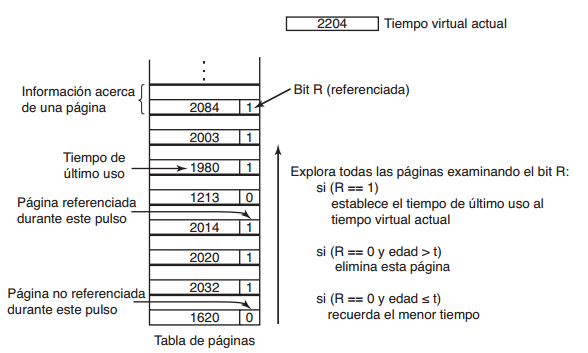
\includegraphics[scale=0.7]{img/workingset.png}
	\caption{Algoritmo Working Set}
\end{figure}


%-------------------------------------------------------------%
{\centering \section*{Algoritmo WS Clock}}
Este algoritmo mezcla el Working Set con el Clock. Se usa una lista circular, cada entrada contiene el campo tiempo de ultimo uso y el bit $R$ y el $M$.

Al ocurrir un fallo de pagina se examina la página a la se esta apuntando (como la manecilla del reloj), Si el bit $R$ es 1, la página se ha utilizado durante el pulso actual, por lo que no es candidata ideal para la eliminación. Después el bit $R$ se establece en 0, la manecilla se avanza a la siguiente página y se repite el algoritmo para esa página.

Si el bit $R$ es 0, se toma en cuenta la edad. Si la edad es mayor que $\tau$ y la pagina esta limpia, significa que no se encuentre en el conjunto de trabajo y existe una copia valida en el disco. Si la página está sucia no se puede reclamar de inmediato, ya que no hay una copia válida presente en el disco. Para evitar una conmutación de procesos, la escritura al disco se planifica pero la manecilla avanza y el algoritmo continúa con la siguiente página, ya que podría haber una página antigua y limpia más allá de la línea que se pueda utilizar de inmediato.

\begin{figure}[H]
	\centering
	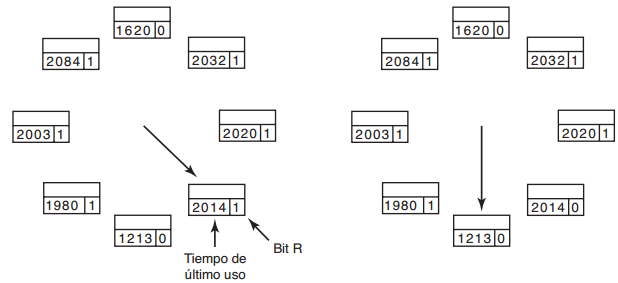
\includegraphics[scale=0.7]{img/wsclock1.png}
\end{figure}

\begin{figure}[H]
	\centering
	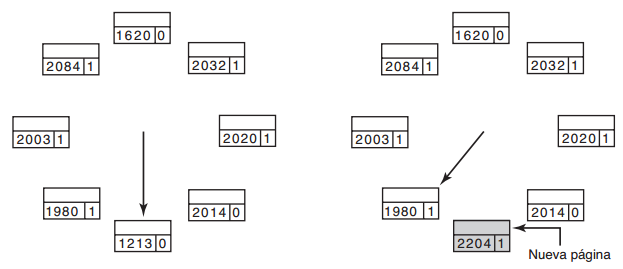
\includegraphics[scale=0.7]{img/wsclock2.png}
	\caption{Algoritmo WS Clock con tiempo virtual actual = 2204}
\end{figure}


%-------------------------------------------------------------%
{\centering \section*{Anomalia de Belady}}
La anomalía de Belady es un efecto descubierto y demostrado en 1969 por el científico de la computación húngaro Laszlo Belady, por el cual es posible tener más fallos de página al aumentar el número de marcos en la memoria física utilizando el método FIFO como algoritmo de reemplazo de páginas en sistemas de gestión de memoria virtual con paginación. Antes de esta fecha, se creía que incrementar el número de marcos físicos siempre llevaría a un descenso del número de fallos de página o, en el peor de los casos, a mantenerlos. Así, pues, antes del descubrimiento de la anomalía de Belady, el algoritmo FIFO era aceptable.


%-------------------------------------------------------------%
{\centering \section*{Distancia de la cadena}}
En el caso de los algoritmos de pila, para cada elemento en la cadena de referencia, la distancia de la cadena representa la distancia de ese elemento desde el tope de la pila.


%-------------------------------------------------------------%
{\centering \section*{Prediccion de la tasa de fallos}}
La cadena de distancias se usa para predecir el numero de fallos de pagina que se presentaran con memorias de diferente tamaño. Lo primero que hace el algoritmo es explorar la cadena de distancias, pagina por pagina, llevando la cuenta de las veces que aparece cada numero. Se denota como $C_{i}$ el numero de veces que aparece $i$. Luego calculamos con la formula 

\begin{equation*}
	F_{m} = \sum_{k=m+1}^{n}C_k + C_\infty
\end{equation*}

El valor de $F_{m}$ es el numero de fallos de pagina que se presentaran con la cadena de distancias dada y $m$ marcos de pagina. $C_\infty$ es el numero de veces que aparece $\infty$ en la cadena de distancias.

\begin{figure}[H]
	\centering
	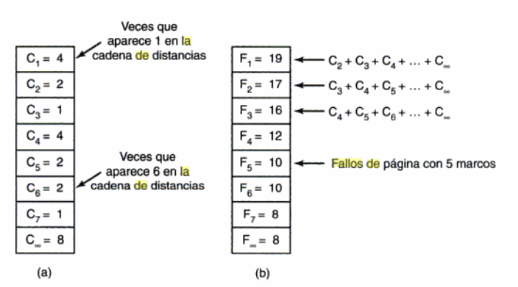
\includegraphics[scale=1]{img/fallos.png}
\end{figure}
%--% Bibliografia %-------%
%\newpage
%\nocite{*}
%\bibliographystyle{unsrt}
%\bibliography{bibliography}
%--------------------------%
\end{document}
